\documentclass{article}
\usepackage[utf8]{inputenc}
\usepackage{fancyhdr}
\usepackage{graphicx}
\usepackage{geometry}
\usepackage{float}

% ---- Commands ------- %
\newcommand{\documentNumber}[1]{
    \LARGE  \textbf{ Kravspecifikation }
    \\
    \medskip
}
\newcommand{\documentVersion}[1]{
    \medskip
}
\newcommand{\documentTitle}[1]{
    \centerline{\rule{13cm}{0.4pt}}
    \bigskip \bigskip
    \LARGE \textbf{Projekt IDA3} \\
    \bigskip
    \LARGE {#1} \\
    \bigskip \bigskip
    \centerline{\rule{13cm}{0.4pt}}
}

\newcommand{\documentDate}[1]{
    \date {#1} 
}


\renewcommand{\arraystretch}{1.7}  % Vertical padding for tables

\renewcommand{\contentsname}{Innehållsförtäckning}

% --- Header & Footer ---- %
\pagestyle{fancy}
\lhead{\leftmark}
\rhead{}
\rfoot{\thepage}
\cfoot{}
\lfoot{}


% ------------------------------------------------ #

% ----- FILL THIS ----- %
\title {
    \documentNumber {01}    

    % Full name - SHORTNAME
    \documentTitle {Helsingborg Event and Convention Bureau}
    
    % Format: YYYY-MM-DD
    \documentDate {2021-08-20}
    \documentVersion Vv 0.2
    
    \author{Anna Bergvall - Oscar Blixt - Pontus Persson - Filip Sjövall - David Vilppu}
}

\begin{document}
\addtocontents{toc}{\protect\setcounter{tocdepth}{2}}
\maketitle

\thispagestyle{empty}



\newpage

\tableofcontents


\newpage

\section{Dokumenthistoria}
\begin{tabular}{ l | l | l }
    Version & Date & Description \\
    \hline
    0.1 & 2021-10-06 & Dokumentet skapat. \\
    0.2 & 2021-11-05 & Första utkast\\
    
\end{tabular}

\section{Introduktion}

    Detta dokument innehåller kraven för ett rapporteringssystem som hädanefter benämns som "systemet". Sysemet är framtaget och utvecklat på beställning av Helsingborg Convention and Event Bureau (HCEB). Det huvudsakliga syftet med systemet är att Helsingborg stad ska bli miljöcertifierat av GDSM (Global Destination Sustainability Movement) genom att inkorporera deras krav för miljöcertifiering i ett frågeformulär som näringslivet får svara på. Huvudfunktionaliteten är att HCEB ska kunna sammanställa den data som tillkommit till följd av svar på formuläret från näringslivet. Systemet ska interageras i en server och det är detta som ska levereras till kunden. I systemet ingår frontend/hemsidan(html, css, javascript), api:n samt databasen. 
    \\\\
    Dokumentets struktureras utifrån prioritering och numrering. Numrering sker enligt \textit{R1} vilka är krav som endast kan hittas i detta dokument, krav med numrering enligt \textit{SF} kommer från scrumboarden. Kraven är prioriterade utefter \textit{stabila krav}, \textit{ändringsbenägna krav} och \textit{uteslutna krav}. 
    

\section{Bakgrund och mål}
                                                                                                                
    \subsection{Mål}
      Helsingborg stad önskar bli certifierade av nätverket Global Detination Sustainability Movement (GDSM), vilket kräver att destinationen varje år skickar in information om hållbarhetsarbetet som utförs av aktörer verksamma inom besöksnäringen i regionen. Syftet med det här projektet är att hjälpa Helsingborg stad att samla in dennahållbarhetsdata genom att utveckla ett webbaserat frågeformulär som går snabbt och är enkelt att svara på. När datan väl samlats in är det vår uppgift att ta fram en sammanställning som matchar GDSM:s målformat. 
        
    \subsection{Viktiga aktörer}
    Systemet kommer ha två typer av användare:
    \begin{itemize}
        \item \textbf{Svarspersoner:} De personer som jobbar på företagen till vilka frågorna riktar sig. Svarspersonerna kommer att logga in med sin mailadress och svara på formuläret.
        \item \textbf{Admin:} HCEB ska tilldelas rollen administratör och således ha tillgång till en administrationssida där de kan sammanställa årets hållbarhetsdata på ett sätt som matchar GDSM:s målformat och även se enskilda aktörers svar.
     \end{itemize}
    
    \section{Terminologi}
    \begin{itemize}
        \item \textbf{Administratör:} Administratören har tillgång till systemets alla funktioner.
         \item \textbf{Frågeformulär:} Ett webbaserat system som innehåller frågor med flervalsalternativ samt statistikföring över svaren.
        \item \textbf{HCEB:} Förkortning av Helsingborg Convention and Event Bureau, beställare av systemet.
        \item \textbf{Session:} Data som sparas under tiden som slutanvändaren befann sig på hemsidan.
        \item \textbf{Svarspersoner och slutanvändare:}  De personer som svarar på frågeformuläret, vilka främst arbetar inom besöksnäringen i Helsingborgs stad. 
        \item\textbf{Stabila krav:}  Stabila krav är krav som inte är ändringbenägna - de baseras på funktioner som är grundläggande för att systemet ska möta beställarens behov.
         \item \textbf{Uteslutna krav:}  Krav som inte längre är aktuella.
        \item \textbf{Ändringbenägna krav:}  Krav som sannolikt kommer att förändras eller tas bort.
       
    \end{itemize}
    \newpage
    \section{Hemsidans design}
    
    \subsection*{Stabila krav}
     
    \subsection*{Ändringsbenägna krav}
     \subsubsection*{R1}
    Systemet ska ha ett utseende likt figur 1.
    
    \begin{figure}[h!]
    \caption{Prototyp över frågeformuläret}
    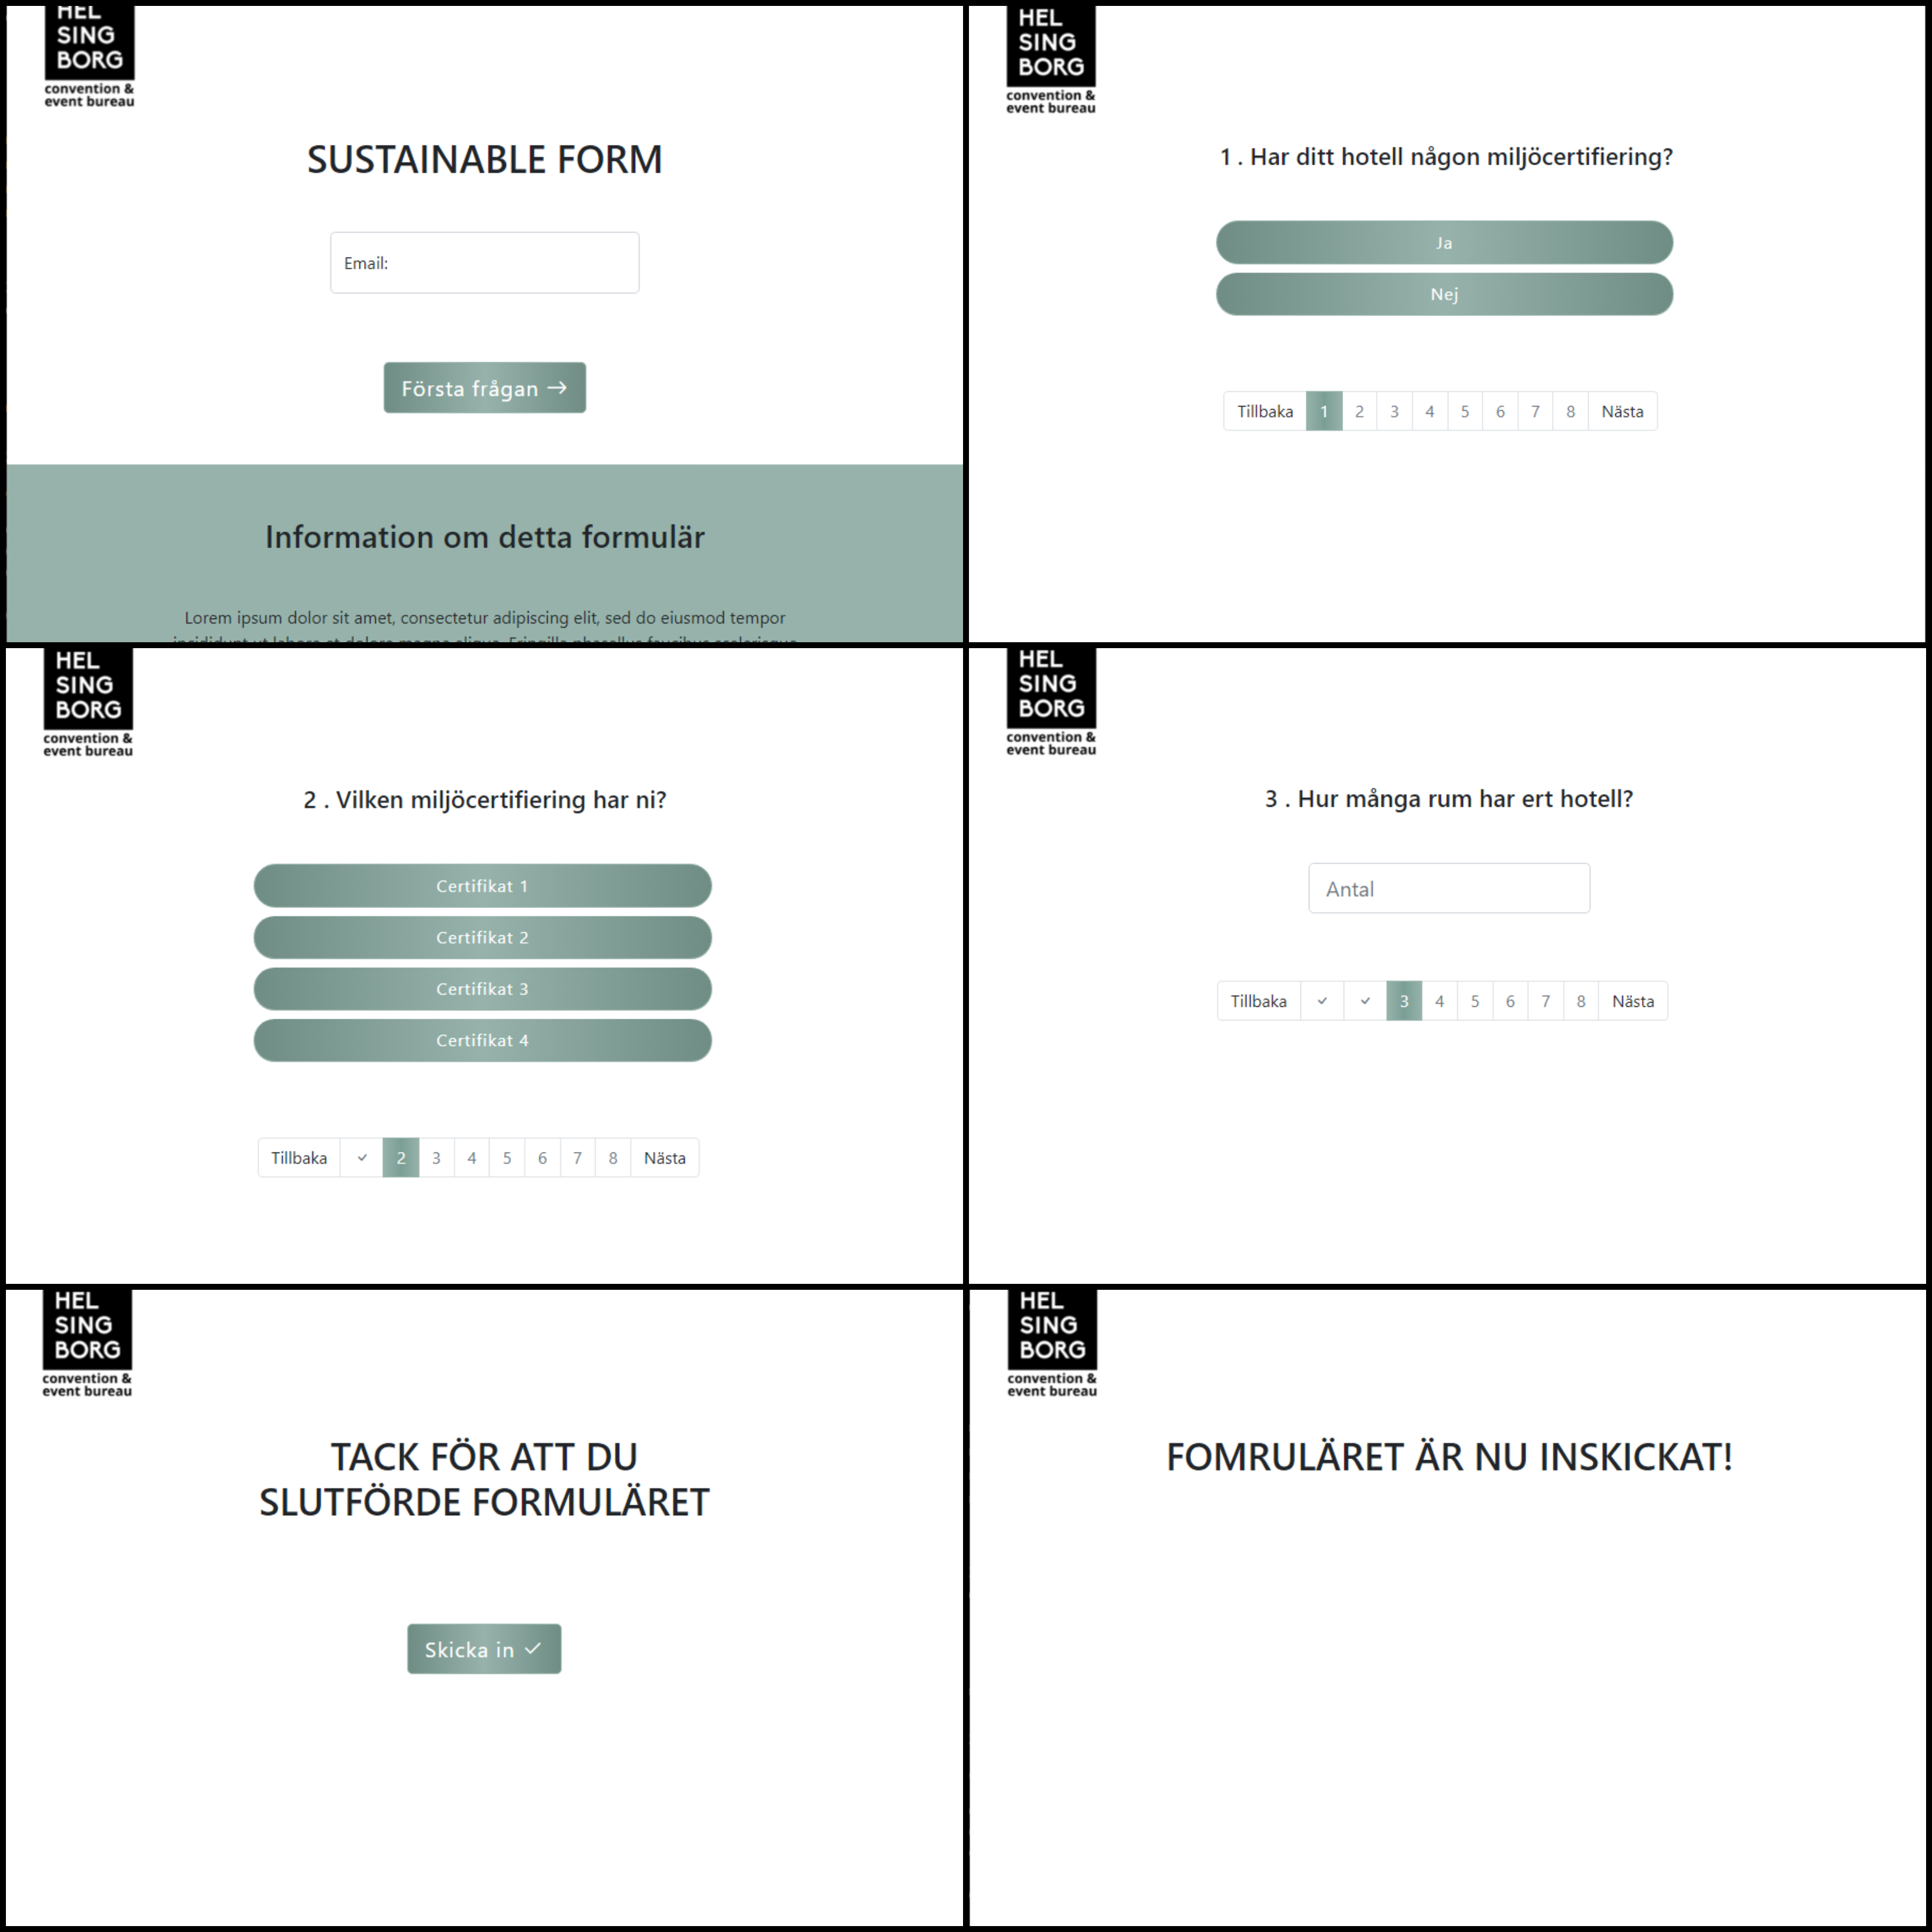
\includegraphics[width=140mm]{Proto-Coll-Q (1).jpg}
    \end{figure}
    \newpage
    \subsubsection*{R11}
    Systemet ska ha ett utseende likt figur 2.
    \begin{figure}[h!]
        \centering
        \caption{Prototyp över administratörens sida}
        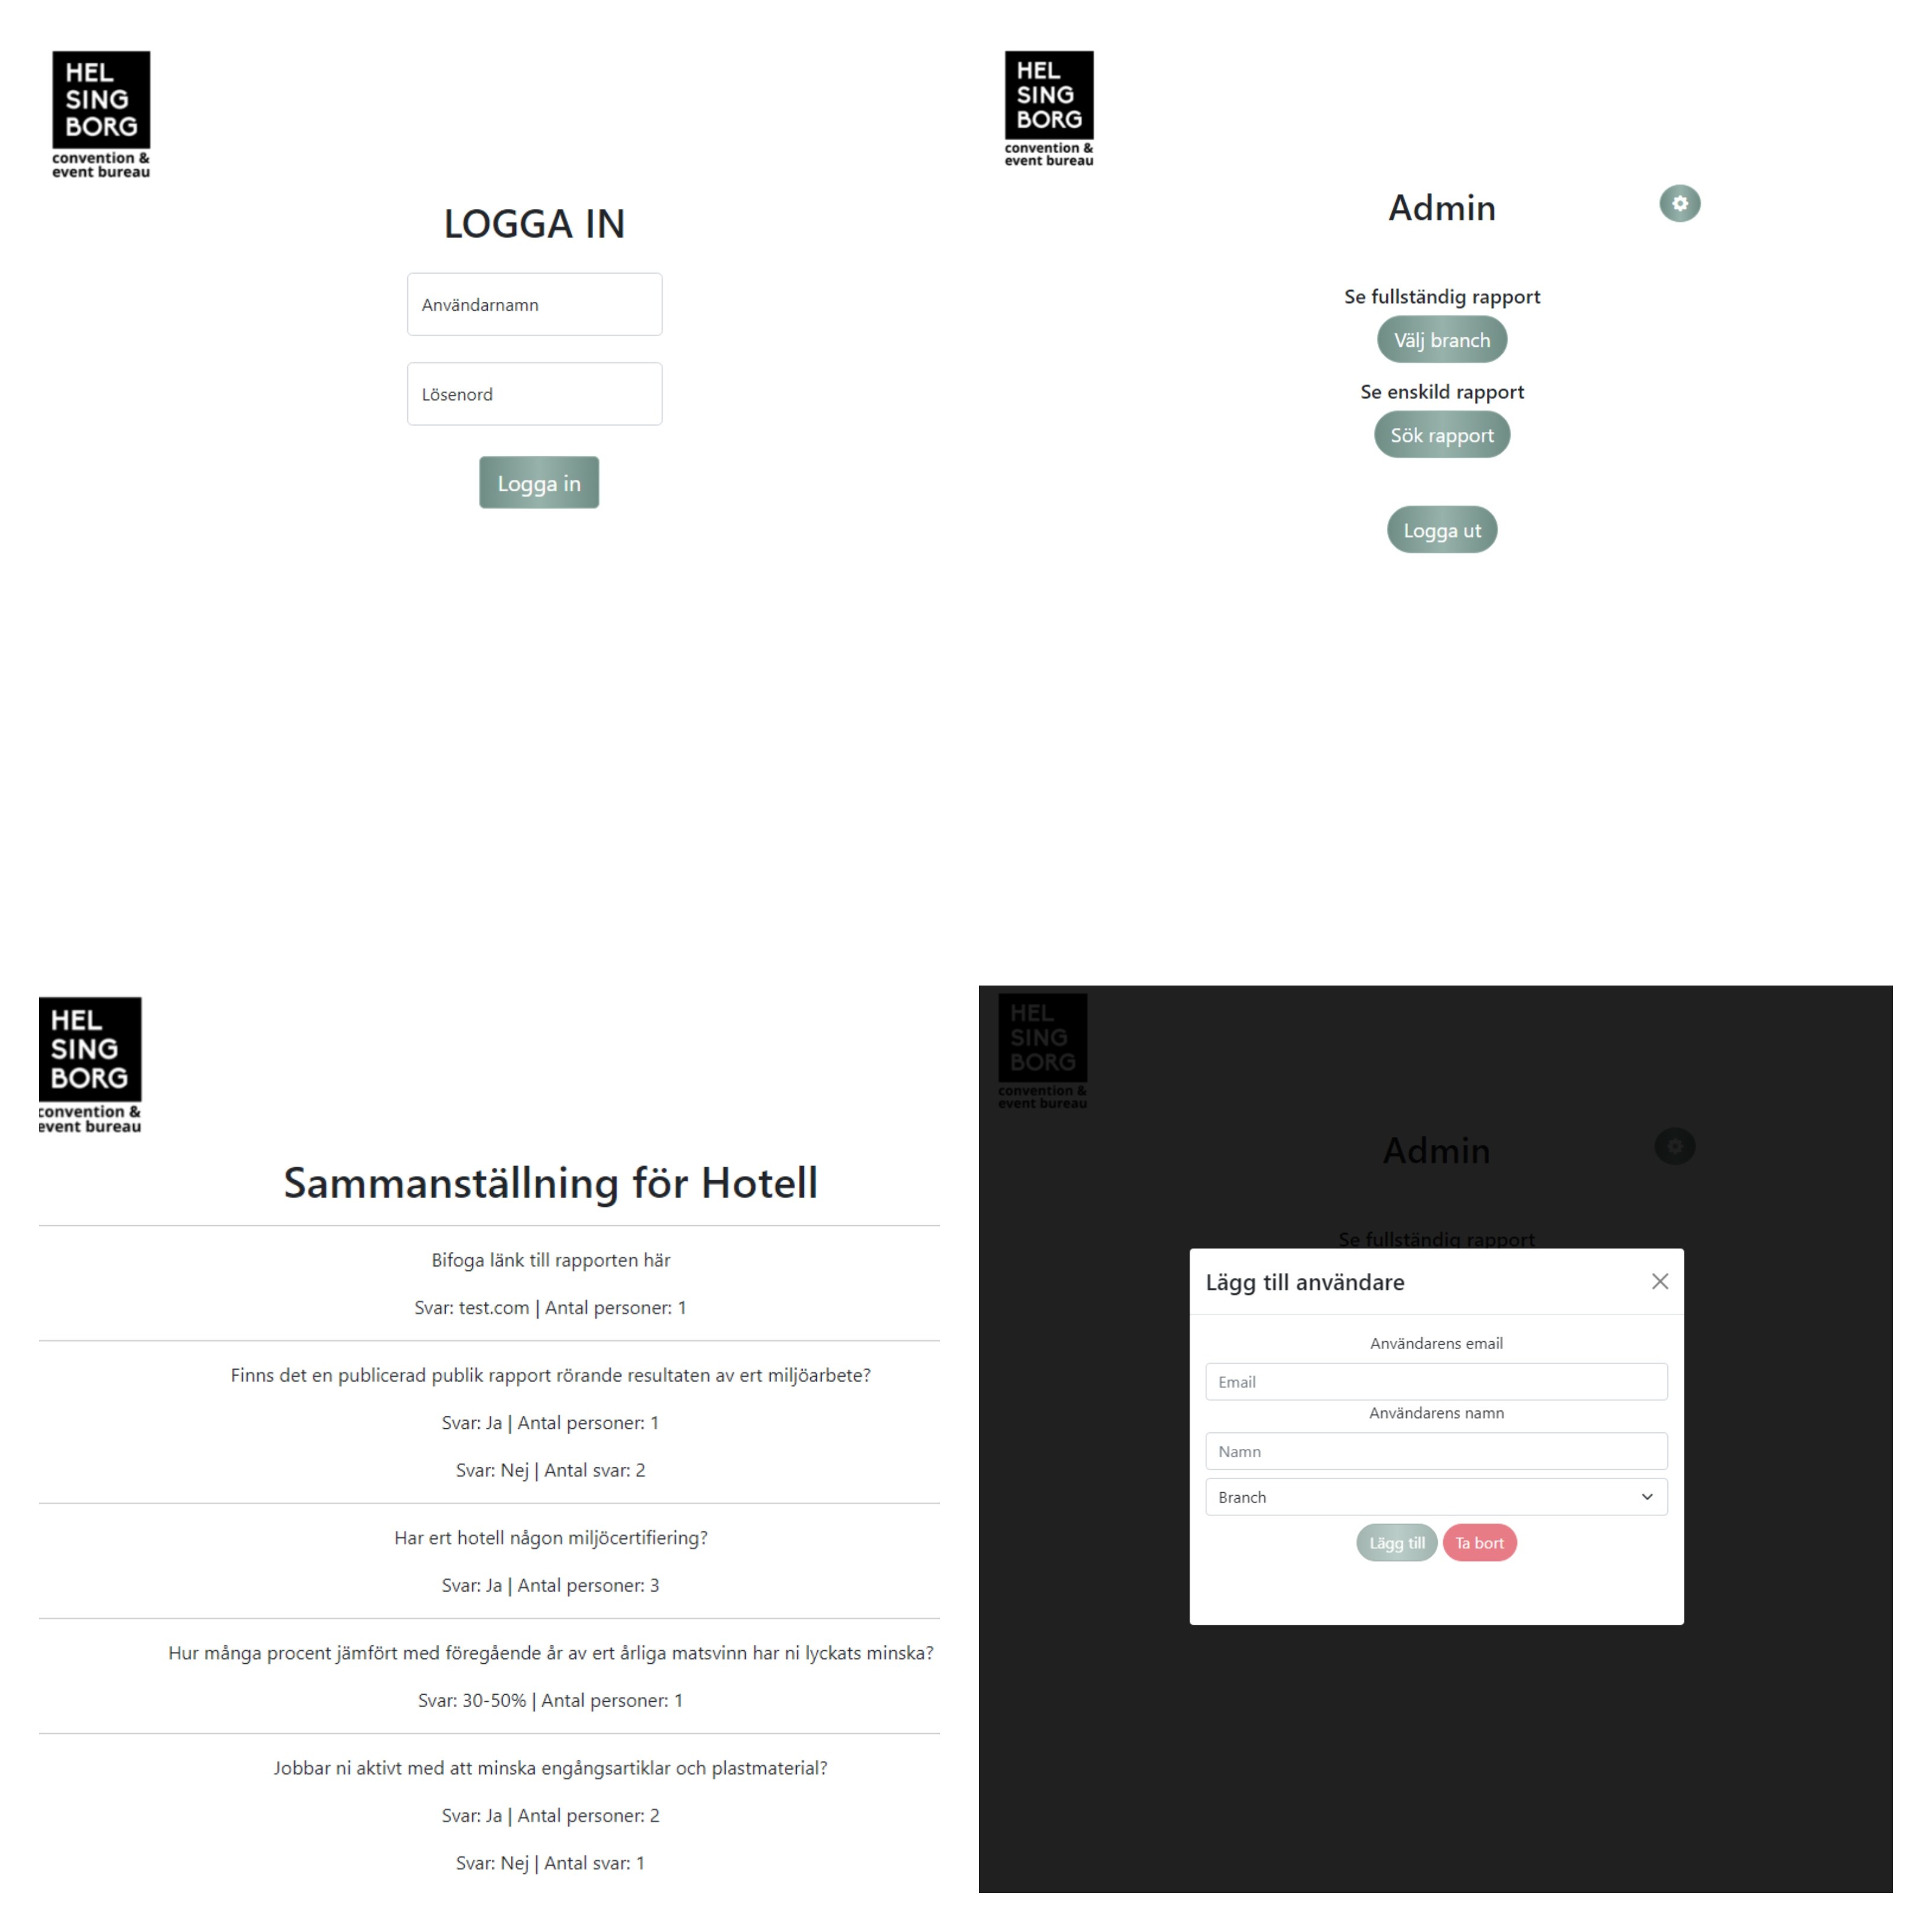
\includegraphics[width=140mm]{Proto-Coll-A.jpg}
        \label{fig:my_label}
    \end{figure}

    \subsection*{Uteslutna krav}
    
    \section{Hemsidans funktion}
    
    \subsection*{Stabila krav}
    
      \subsubsection*{R2}
    Följande scenario ska stödjas av systemet.
        \\
       \indent \textbf{Scenario:} Slutanvändaren navigerar till hemsidan via mail.
        \\
       \indent \textbf{Förutsättningar:} Svarspersonen har fått ett mail från från HCEB. Mailet innehåller en länk till hemsidan.
            \begin{enumerate}
                \item Slutanvändaren klickar på länken till formuläret som finns i mejlet.
                \item Slutanvändaren möts av formulärets startsida och ombeds mata in sin mailadress till vilken länken skickades. 
            \end{enumerate}
            
        \subsubsection*{R3}
    Följande scenario ska stödjas av systemet.
        \\
       \indent \textbf{Scenario:} Slutanvändaren ska logga in på hemsidan med sin samma mailadress som mailet skickades till.
        \\
       \indent \textbf{Förutsättningar:} Svarspersonen har fått en engångskod i samma mail som länken samt att svarspersonen befinner sig på startsidan.
            \begin{enumerate}
               \item Svarspersonen skriver in samma mailadress som mailet skickades till.
               \item Svarspersonen trycker på knappen "Gå vidare".
                \item  Svarspersonen blir omdirigerad till första frågan och kan börja svara på formuläret.
            \end{enumerate}
   
        \subsubsection*{R4}
    Följande scenario ska stödjas av systemet.
        \\
       \indent \textbf{Scenario:} Svarspersonen ska skicka in slutgiltig rapportering.
        \\
       \indent \textbf{Förutsättningar:} Svarspersonen har svarat på samtliga frågor och befinner sig på sidan med den sista frågan.
            \begin{enumerate}
                \item Svarspersonen klickar på knappen "Slutför formulär".
                \item Svarspersonen möts av en sidan med tack text enligt figur 1.
                \item Svarspersonen trycker på knappen "Skicka in formulär".
                \item  Svarspersonen möts av en bekräftelsesida som bekräftar att formuläret är inskickat.
            \end{enumerate}

\subsection*{Ändringsbenägna krav}

\subsubsection*{Krav från scrumboard}
Följande mappning gäller för de krav som finns på projektets scrumboard som finns på \\
https://trello.com/b/DHOoURT9/sustainable-forms
\\
När ett krav ska refereras till används denna graf.\\
$$SR1\rightarrow SF-1$$
$$SR2\rightarrow SF-5$$
$$SR3\rightarrow SF-6$$
$$SR4\rightarrow SF-7$$
$$SR5\rightarrow SF-9$$
$$SR6\rightarrow SF-12$$
$$SR7\rightarrow SF-22$$
$$SR8\rightarrow SF-13$$
$$SR9\rightarrow SF-14$$
$$SR10\rightarrow SF-16$$
$$SR11\rightarrow SF-17$$
$$SR12\rightarrow SF-18$$
$$SR13\rightarrow SF-21$$
$$SR14\rightarrow SF-25$$
$$SR15\rightarrow SF-64$$
$$SR16\rightarrow SF-65$$
$$SR17\rightarrow SF-73$$
$$SR18\rightarrow SF-74$$

    \subsection*{Uteslutna krav}
    
    \newpage
     \section{Hemsidans hantering av data}
    
    \subsection*{Stabila krav}
    \subsubsection*{R5}
    Systemet ska fungera enligt figur 2.
    
    \begin{figure}[h!]
    \caption{Kontext-diagram: Det utvecklade systemet innefattar \textit{Server, API, GUI} och \textit{Systemet}}
    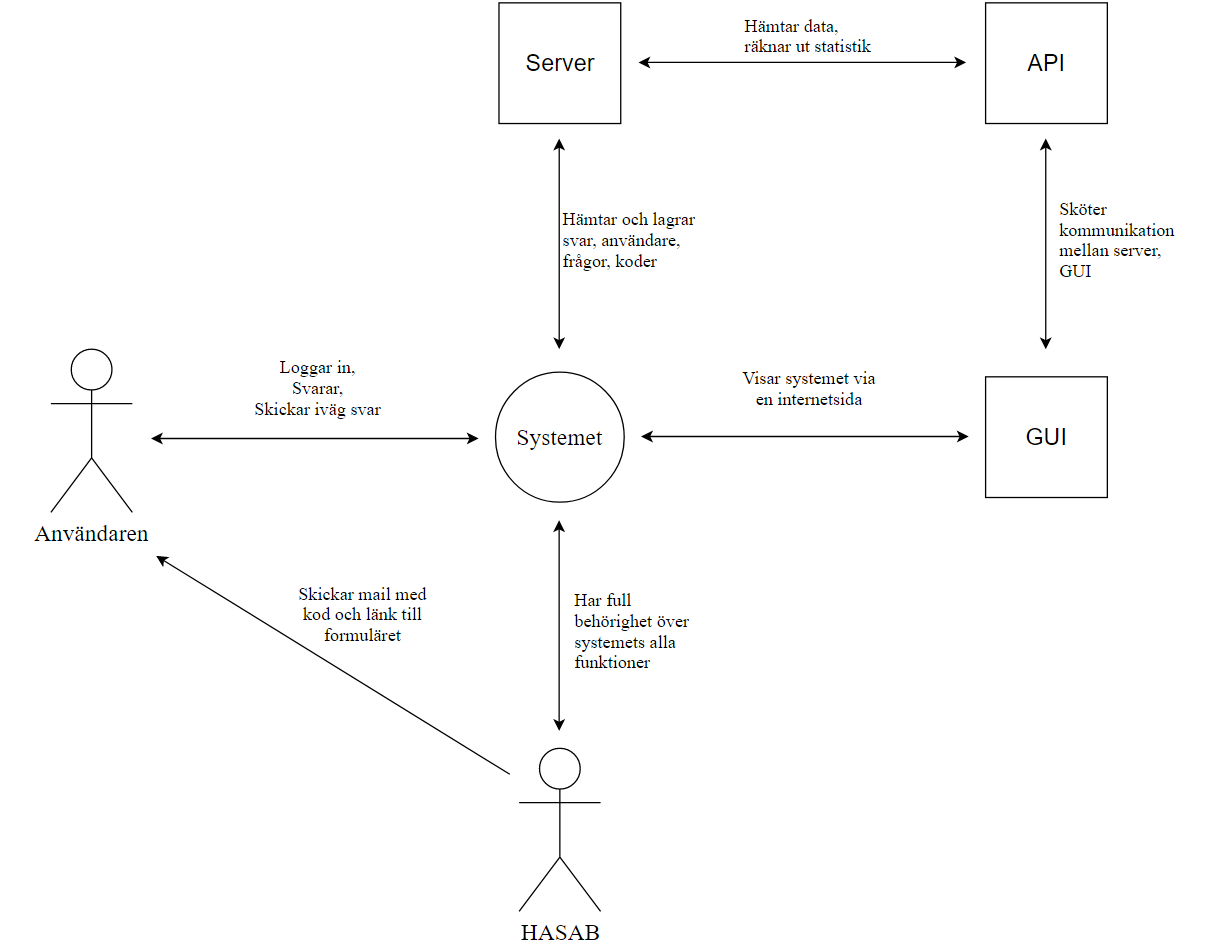
\includegraphics[width=150mm]{Kontextdiagram.png}
    
    \end{figure}
    
    \newpage
    \subsubsection*{R6}
    Systemt ska hantera data enligt figur 3.
       \begin{figure}[h!]
    
    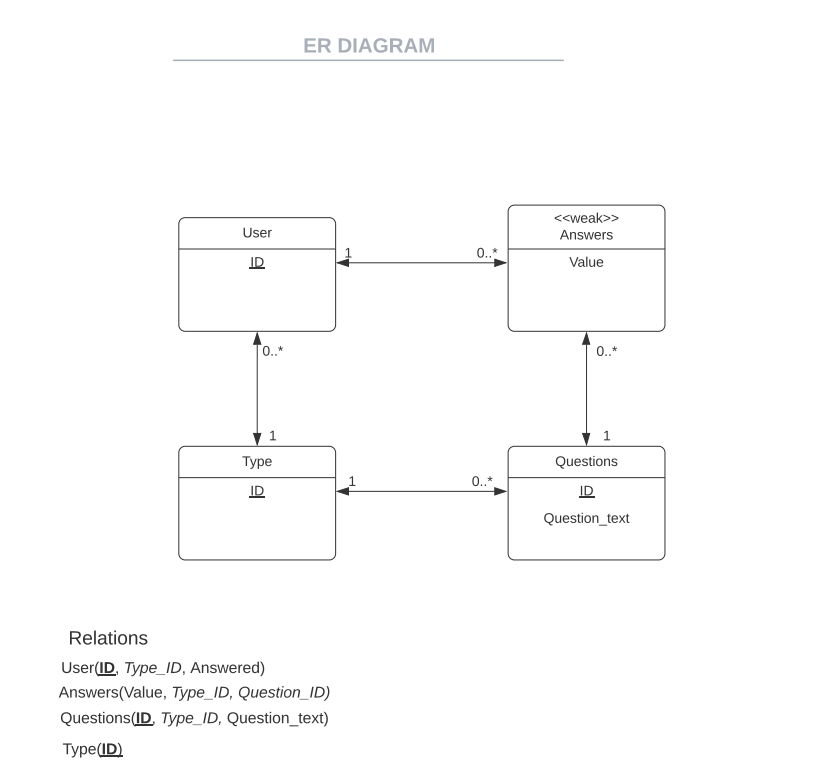
\includegraphics[width=150mm]{ERDIAGRAM.png}
    \caption{ER-Diagram}
    \end{figure}
    
    \newpage
    \subsection*{Ändringsbenägna krav}
    \subsection*{Uteslutna krav}
    
  
   
    \section{Kvalitetskrav}
    \subsection*{Stabila krav}
    
  
     \subsection*{Ändringsbenägna krav}
     \subsubsection*{R6}
     Vid oförutsebara händelser som påverkar systemets tillgänglighet ska en session sparas i 24 timmar från att den påbörjades.
     
     \subsubsection*{R7}
    Systemet ska ha en svarstid på max \underline{\hspace{1cm}} sekunder.
    
    \subsubsection*{R8}
    Rapportering i systemet ska endast kunna göras av en användare som har fått tillgång till hemsidan via mail.
    
     
    \subsubsection*{R10}
    Fyra av fem användare ska anse att enkäten var lätt att svara på.
    
    \subsubsection*{R11}
    En medelkunnig slutanvändare ska kunna genomföra scenariot som beskrivs i \textbf{R2} och anlända till sidan inom 20 sekunder efter att de har klickat på länken.
    
    \subsubsection*{R12}
    En medelkunnig slutanvändare ska kunna genomföra scenariot som beskrivs i \textbf{R3} inom en minut.
    
    \subsubsection*{R13}
    En medelkunnig slutanvändare ska kunna genomföra scenariot som beskrivs i \textbf{R4} inom 20 sekunder.
    
    \subsection*{Uteslutna krav}
    
    \section{Leveranskrav}
    
    \subsection*{Stabila krav}
     \subsubsection*{R14}
     En leverans av systemet ska ske 2021-12-13 och ska inludera en fungerande produkt som kan användas för testning av kunden.
     
     \subsubsection*{R15}
     Slutgiltig leverans av systemet ska ske 2021-12-13 och ska inkludera en fullt fungerade produkt.
     
     
    \subsection*{Ändringsbenägna krav}
    
    \subsection*{Uteslutna krav}
    
    
   
\bibliographystyle{alpha}


\end{document}
